Exécution du programme avec le fichier suivant:
\inputminted[frame=single,label=Test]{text}{../tests/test_insert}

\begin{figure}[h!]
	\centering
	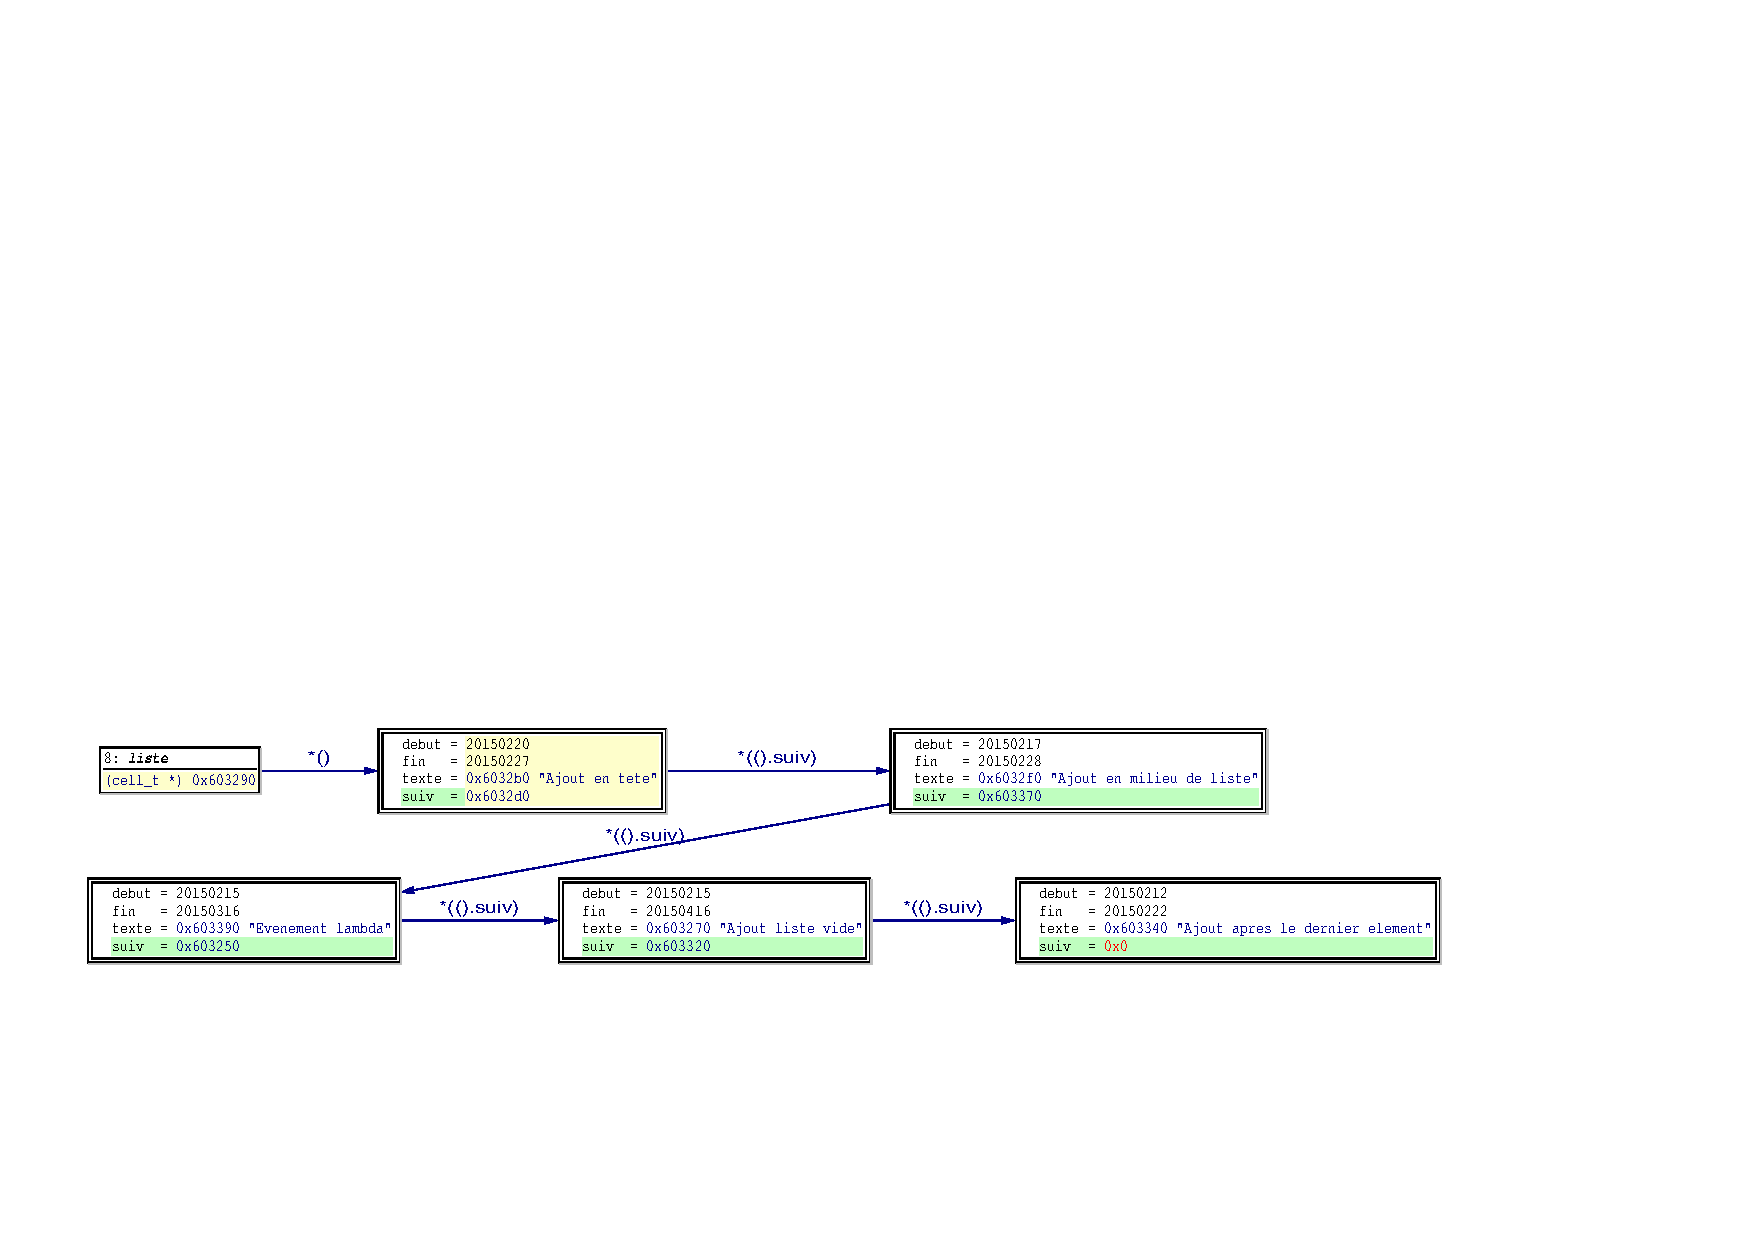
\includegraphics[width=18cm,clip=true,trim=1cm 4cm 5cm 12cm]{../tests/ddd_graph/chargement}
	\caption{Après lecture du fichier, contenu de \texttt{liste}}
\end{figure}

\begin{figure}[h!]
	\centering
	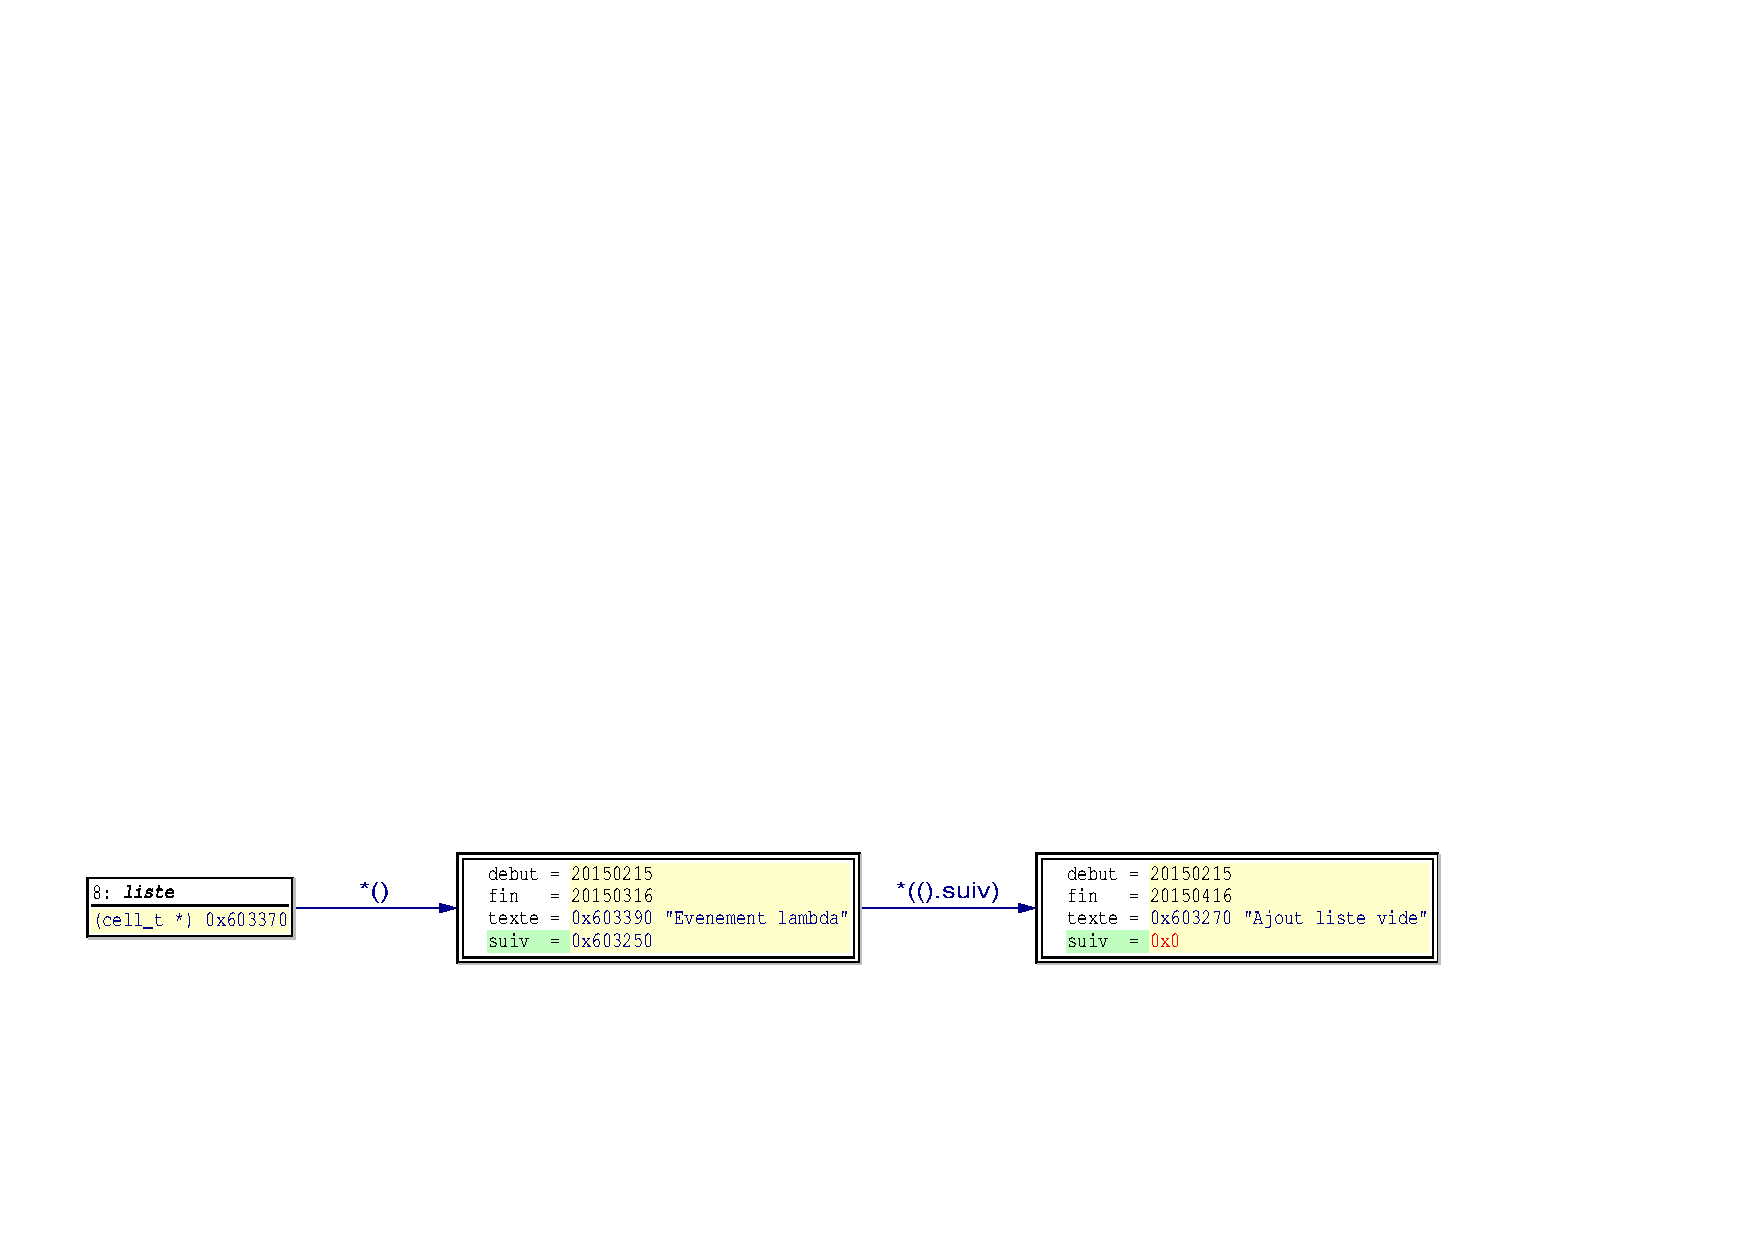
\includegraphics[width=15cm,clip=true,trim=1cm 4cm 5cm 13cm]{../tests/ddd_graph/nettoyage}
	\caption{Après suppression des messages obsolètes, contenu de \texttt{liste}}
\end{figure}

\begin{figure}[h!]
	\centering
	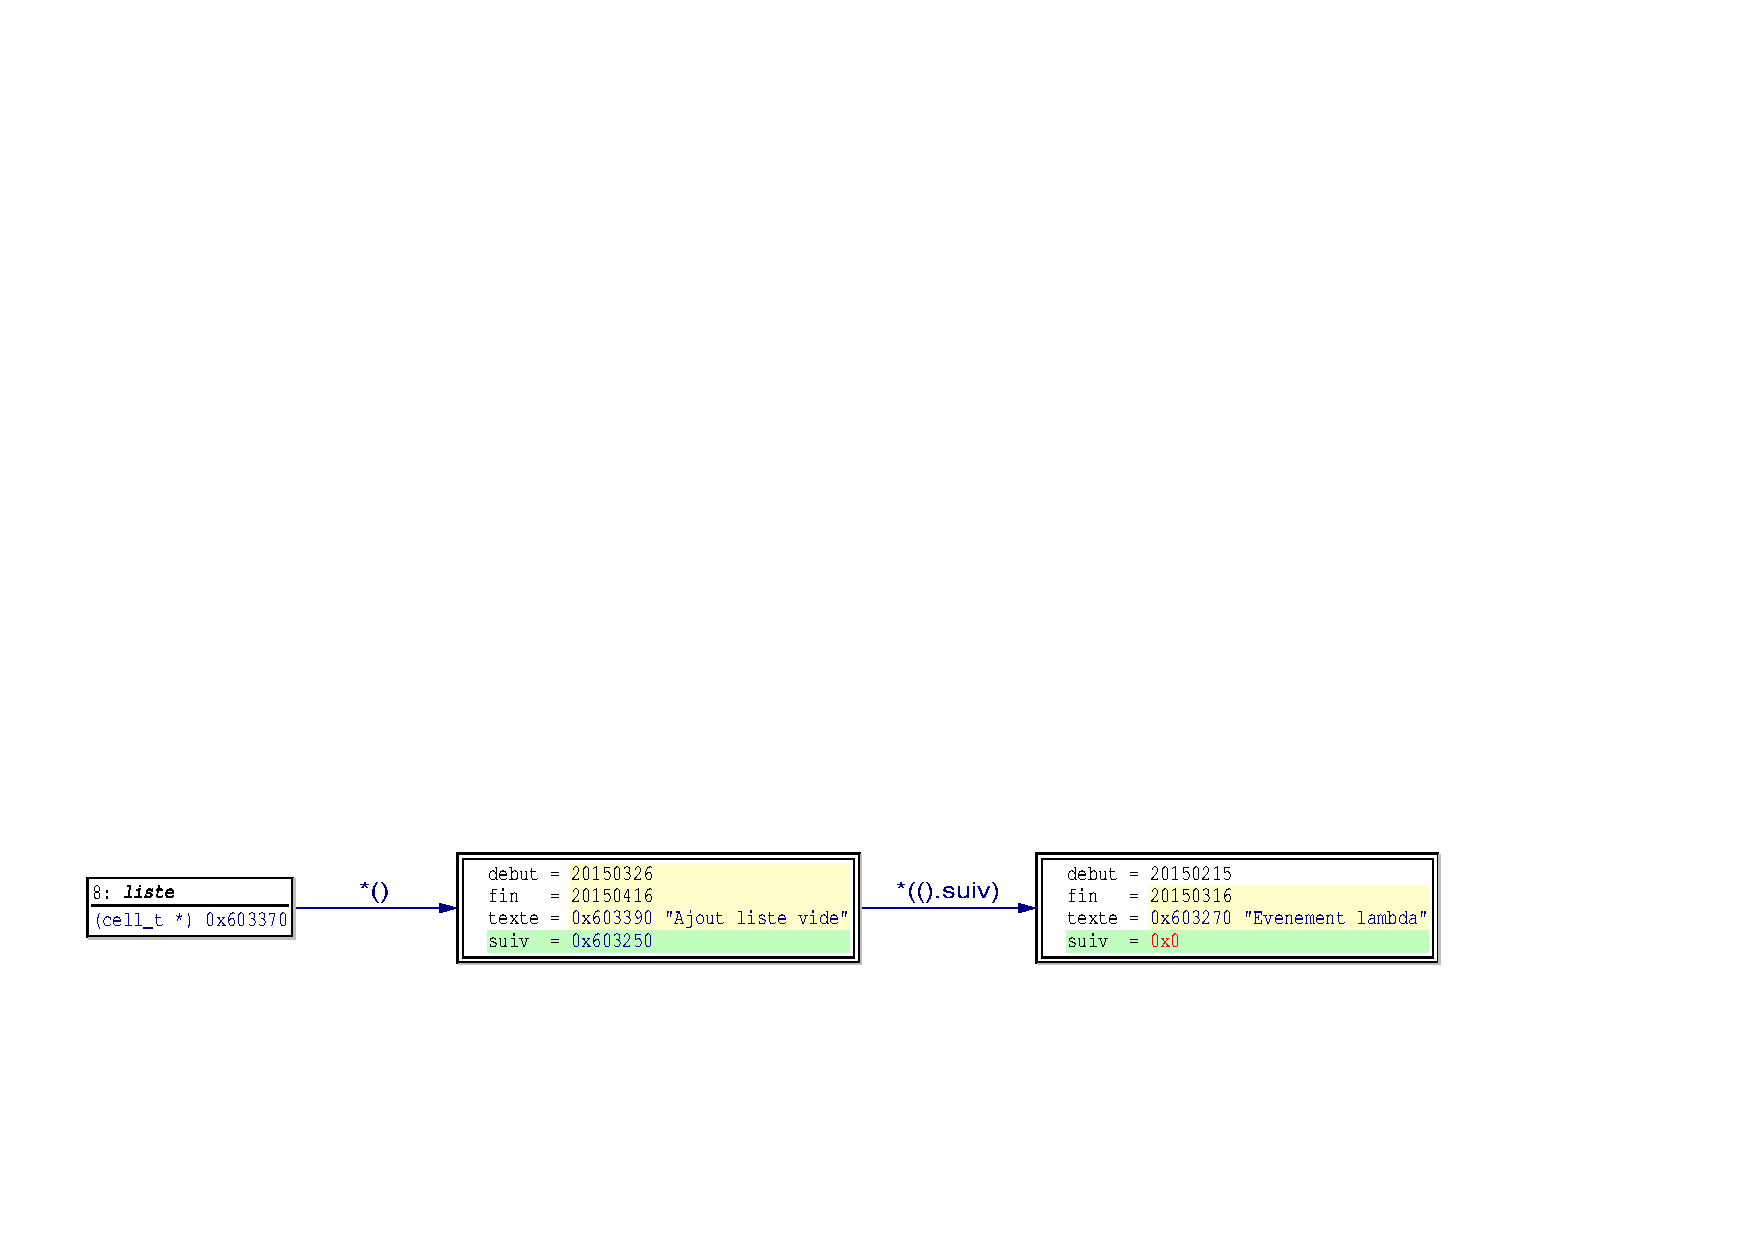
\includegraphics[width=15cm,clip=true,trim=1cm 4cm 5cm 13cm]{../tests/ddd_graph/modification}
	\caption{Après modification de date de début, contenu de \texttt{liste}}
\end{figure}

\begin{figure}[h!]
	\centering
	
\includegraphics[width=3cm,clip=true,trim=1cm 4.5cm 25cm 15cm]{../tests/ddd_graph/suppression}
	\caption{Après suppression de la liste, contenu de \texttt{liste}}
\end{figure}

\begin{figure}[h!]
	\centering
	\inputminted[frame=single,label=Terminal]{text}{../tests/resultat_test_insert}
	\caption{Exécution du programme sur la sortie standard}
\end{figure}

\begin{figure}[h!]
	\centering
	\inputminted[frame=single,label=Terminal]{text}{../tests/valgrind_report}
	\caption{Exécution avec valgrind}
\end{figure}
%\fbox{